\section{The \textbf{TransP-0} integrated design abstraction}
\label{proposed_model}

The \textsc{TransP-0} design abstraction is intended to support both transportation and power system engineers during early project phases in formulating and evaluating different design options quickly. Therefore, transportation and power system properties - both static and dynamic - have to be captured sufficiently precise. On the other hand, the design abstraction should omit unnecessary details to enable frequent design iterations. With these requirements in mind we have developed a candidate design abstraction, which is summarized in Figure~\ref{system_design}. The abstraction comprises various transportation and a power respectively energy subsystem parameters as well as subsystem-specific and -spanning constraints and objectives.

\begin{figure}[h!]
	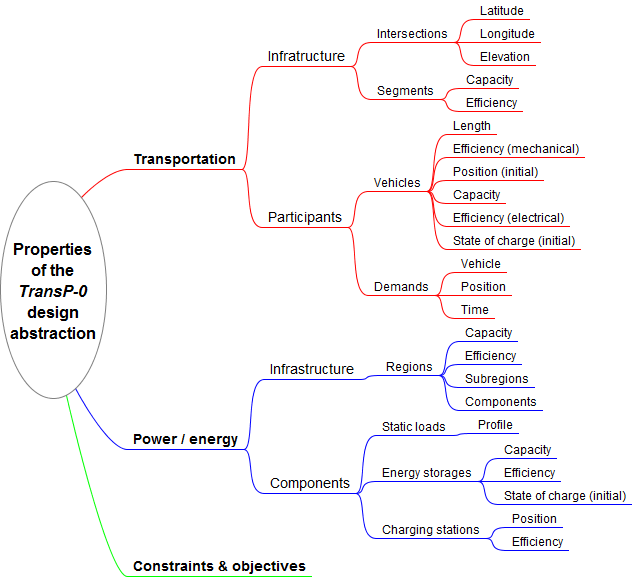
\includegraphics[width=\columnwidth]{./gfx/system_design.png}
	\caption{\textsc{TransP-0} integrated design abstraction comprising various transportation subsystem and power subsystem parameters as well as subsystem-specific and -spanning constraints and objectives.}
	\label{system_design}
\end{figure}

In the following, we first describe the design abstraction for the transportation subsystem in Section~\ref{transport} and the power respectively energy subsystem in Section~\ref{energy_system}. Then, we explain the subsystem-specific and -spanning constraints in Section~\ref{constraints} as well as the objectives in Section~\ref{objectives}. 

\subsection{Transportation subsystem}
\label{transport}

The transportation subsystem $TS$ of the integrated design abstraction is modeled as a tuple
\[
	TS = (TSI, TSP) \textrm{,}
\]
where $TSI$ represents the transportation infrastructure (i.e.\ roads and their intersections) and $TSP$ represents the individual traffic participants (i.e.\ passenger cars and goods vehicles). In the following, we describe the the infrastructure design abstraction in Section~\ref{transport_infrastructure} before explaining the participant design abstraction in Section~\ref{participants}.

\subsubsection{Infrastructure}
\label{transport_infrastructure}

The transportation subsystem infrastructure $TSI$ of the transportation subsystem $TS$ is modeled as a tuple
\[
	TSI = (RI, RS) \textrm{,}
\]
where $RI$ represents road intersections and $RS$ represent road segments. Subsequently, we first describe the road intersections in Section~\ref{intersections} before explaining the road segments in Section~\ref{segments}.

\paragraph{Intersections}
\label{intersections}

The road intersections $RI$ of the transportation subsystem infrastructure $TSI$ are modeled - again - as a tuple
\[
	RI = (RIL, RIC) \textrm{,}
\]
where $RIL$ represents a finite set of road intersection labels and $RIC$ represents a mapping from road intersection labels $RIL$ to geometric coordinates
\[
	RIC: RIL \rightarrow \mathbb{R}^3 \mathrm{.}
\]
Note that typically the coordinates are expressed in terms of latitude, longitude, and elevation. However, for simplicity in this work we use Cartesian coordinates instead. Consequently, distances can be computed more easily using the Euclidean metric. Moreover, transformations exist to switch between polar and Cartesian coordinates.

\paragraph{Segments}
\label{segments}

In contrast, the road segments $RS$ of the transportation subsystem infrastructure $TSI$ are modeled as a five-tuple
\[
	RS = (RSL, RSS, RST, RSC, RSE) \textrm{,}
\]
where $RSL$ represents a finite set of road segment labels, $RSS$ and $RST$ represent mappings from road segment labels $RSL$ to their respective source and target road intersection labels $RIL$
\[
	RSS/RST: RSL \rightarrow RIL \textrm{,}
\]
$RSC$ represents a mapping from road segment labels $RSL$ to the number of lanes (i.e.\ the \textit{capacity} of the road segment)
\[
	RSC: RSL \rightarrow \mathbb{N} \textrm{,}
\]
and $RSE$ represents a mapping from road segment labels $RSL$ to their surface material (i.e.\ the \textit{efficiency} of the road segment)
\[
	RSE: RSL \rightarrow \mathbb{R}^+ \textrm{.}
\]
Note that the previous parameters completely determine our road segment model. Consequently, we abstract from a variety of parameters typically considered such as \todo{...}.

Furthermore, we derive the road segment distance $RSD$ as a mapping from road segment labels $RSL$ to distances
\[
	RSD: RSL \rightarrow \mathbb{R}_0^+
\]
and we use the Euclidean metric $E: \mathbb{R}^3 \times \mathbb{R}^3 \rightarrow \mathbb{R}_0^+$ to compute the road segment distance $RSD$ as
\[
	RSD(rsl) = E(RIC(RSS(rsl)), RIC(RST(rsl))) \textrm{.}
\]
Finally, we define road segment positions $RSP$ as tuples of road segment labels $RSL$ and traveled distances
\[
	RSP = \{(rsl, d) \in RSL \times \mathbb{R}_0^+ \mid d \leq RSD(rsl)\} \textrm{.}
\]
We use the road segment positions $RSP$ to locate traffic participants (i.e.\ vehicles) on the transportation subsystem infrastructure $TSI$ as explained in Section~\ref{participants}.

\subsubsection{Participants}
\label{participants}

The transportation subsystem participants $TSP$ of the transportation subsystem $TS$ are modeled - again - as a tuple
\[
	TSP = (V, D) \textrm{,}
\]
where $V$ represents the vehicles and $D$ represents the demands. In the following, we first describe the vehicle design abstraction in Section~\ref{vehicles} before explaining the demand design abstraction in Section~\ref{demands}.

\paragraph{Vehicles}
\label{vehicles}

The vehicles $V$ of the transportation subsystem participants $TSP$ are modeled as seven-tuple
\[
	V = (VL, VS, VME, VP, VC, VEE, VSOC) \textrm{,}
\]
where $VL$ represents a finite set of vehicle labels, $VS$ represents a mapping from vehicle labels $VL$ to their length (i.e.\ the \textit{size} of the vehicle in road segment direction)
\[
	VS : VL \rightarrow \mathbb{R}^+ \textrm{,}
\]
$VME$ represents a mapping from vehicle labels $VL$ to their mechanical efficiency (i.e.\ a constant ratio for the conversion between electrical and mechanical energy)
\[
	VME : VL \rightarrow \mathbb{R}^+ \textrm{,}
\]
$VP$ represents a mapping from vehicle labels $VL$ to their initial road segment positions $RSP$ (see Section~\ref{segments})
\[
	VP : VL \rightarrow RSP \textrm{,}
\]
$VC$ represents a mapping from vehicle labels $VL$ to their battery capacities (i.e.\ the maximum amount of energy that can be stored by the vehicle)
\[
	VC : VL \rightarrow \mathbb{R}^+ \textrm{,}
\]
$VEE$ represents a mapping from vehicle labels $VL$ to their electrical efficiency (i.e.\ a constant ratio for conversion between electrical energy and stored energy)
\[
	VEE : VL \rightarrow \mathbb{R}^+ \textrm{,}
\]
and $VSOC$ represents a mapping from vehicle labels $VL$ to their initial state of charge (i.e.\ the amount of energy stored by the vehicle initially)
\[
	VSOC : VL \rightarrow \mathbb{R}^+ \textrm{ such that } VSOC(vl) \leq VC(vl) \textrm{.}
\]
Note that again we abstract from many parameters typically considered such as \todo{...}. In particular, we approximate mechanical and electrical efficiencies with constants only.

\paragraph{Demands}
\label{demands}

Finally, the demands $D$ of the transportation subsystem participants $TSP$ are modeled as four-tuple
\[
	D = (DL, DV, DP, DT) \textrm{,}
\]
where $DL$ represents a finite set of demand labels, $DV$ represents a mapping from demand labels $DL$ to vehicle labels $VL$ (i.e.\ the concerned vehicle)
\[
	DV: DL \rightarrow VL \textrm{,}
\]
$DP$ represents a mapping from demand labels $DL$ to road segment positions $RSP$ (i.e.\ where the concerned vehicle is expected to be)
\[
	DP: DL \rightarrow RSP \textrm{,}
\]
and $DT$ represents a mapping from demand labels $DL$ to time points (i.e.\ when the concerned vehicle is expected to be there)
\[
	DT: DL \rightarrow \mathbb{N}^+ \textrm{.}
\]
Note that our abstraction is based on discrete time. However, we do not prescribe the time step resolution.

\subsection{Power / energy subsystem}
\label{energy_system}

The energy subsystem $ES$ of the integrated design abstraction is modeled as a tuple
\[
	ES = (ESI, ESC) \textrm{,}
\]
where $ESI$ represents the energy subsystem infrastructure (determined by the transmission and distribution network) and $ESC$ represents energy subsystem components (i.e.\ the actual producers and consumers). In the following, we first explain the infrastructure in Section~\ref{regions} before describing the components in Section~\ref{components}.

\subsubsection{Infrastructure}
\label{energy_infrastructure}

The energy subsystem infrastructure $ESI$ of the energy subsystem $ES$ is modeled as a one-tuple
\[
	ES = (R) \textrm{,}
\]
where $R$ represents the regions of the energy subsystem infrastructure, which are determined by the voltage levels and transformers of the network. Note that we selected a region model~\cite{Hackenberg2012} over a power flow model~\todo{?} to reduce modeling effort and increase computational efficiency. In the following, we describe the regions in Section~\ref{regions}.

\paragraph{Regions}
\label{regions}

Power regions represent an aggregated representation of a set of voltage nets. For example, they can define a region based on specific low, medium or high voltage nets in a given area. However, they abstract from a detailed representation of the underlying physical net structure.  

Hence, the identifier of a power region $PR$ is defined as
\[
\exists n \in \mathbb{N} : |PR| < n \mathrm{.}
\]
Power regions aggregate the loads of their subregions and connected electric devices. In return, they provide the aggregated load to their upper region.
Hence, the acyclic parent relationship with their distinct roots $PRP$ is defined by 
\[
PRP : PR \to PR \mathrm{.}
\]
Power regions are subject to given capacity $PRC$, which describes the total load a power region can aggregate.
The power region capacity $PRC$ is then
\[
PRC : PR \rightarrow \mathbb{R}^+ \mathrm{.}
\]
The current energy balance of a power region
$PRS : PR \rightarrow \mathbb{R}_0^+$ with $cc$ describing the current capacity of an according power region is then
\[
PRS(pr) \in \{ cc \in \mathbb{R}_0^+ \mid 0 \leq cc \leq PRC(pr) \} \mathrm{.}
\]

\subsubsection{Components}
\label{components}

TODO

\paragraph{Static loads}
\label{static_loads}

Static loads represent an aggregation of devices within the power system with non-controllable loads, i.e. energy production or consumption. They are defined by an identifier $SL$, where 
\[
\exists n \in \mathbb{N} |SL| < n \mathrm{.}
\]

Static loads abstract from details regarding specific behavior of specific electric devices. For example, static loads can represent an aggregation of activities with non-controllable loads with human interaction such as cooking or watching television. Based on their selected profile for the given use case, static loads exert different load profiles. Here we consider static loads to be similar to standardized load profiles, which are often utilized by distribution grid operators for different areas of operation such as modeling the load behavior of households, workplaces or agricultural businesses. A given static load profile $SLP$ describes the according load per time instant only, where
\[
SLP : SL \times \mathbb{R}_0^+ \rightarrow \mathbb{R} \times \mathbb{R} \mathrm{.}
\]
Here, static loads are mapped to a specific region, e.g. determining their currently mapped voltage net.

%\paragraph{Energy generators}
%\label{energy_generators}
%
%Power generators represent a class of electric devices which produce load. For example, they can represent conventional energy sources such as fossil-fuel power stations as well as renewable energy sources such as solar panels or wind turbines. For producing energy they take a resource such as coal, gas or sunlight or wind as input. Based on the input, i.e. resource employed, they produce an according output, i.e. positive load and emissions. 
%
%They are defined by an identifier $PG$, where 
%\[
%\exists n \in \mathbb{N} |PG| < n \mathrm{.}
%\]
%Power generators are mapped to specific region, e.g. determining their currently mapped voltage net. Concerning environmental factors, power generator emissions $PGE$ define the total emissions which occur during power production in a time instant.
%\[
%PGP : PG \rightarrow \mathbb{R}_0^+ \mathrm{.}
%\]
%
%Power production is based on their individual power efficiency $SPS$, which defines the total amount of energy they can produce as an output, given a specific resource they utilize.
%\[	
%PGP : PG \rightarrow \mathbb{R}_0^+ \mathrm{.}
%\]
%	
%	Solar panel identifiers $SP$
%	\[
%		\exists n \in \mathbb{N} : |SP| < n
%	\]
%	Solar panel power scale $SPS$ 
%	\[
%		SPS : SP \rightarrow \mathbb{R}^+
%	\]
%	Solar panel power $SPP$ 
%	\[
%		SPP : SP \times \mathbb{R}^+ \rightarrow \mathbb{R}^+
%	\]
%

\paragraph{Energy storages}
\label{energy_storages}

Energy storages can store and release energy at given times. They are defined by an identifier $ES$, where 
\[
\exists n \in \mathbb{N} |ES| < n \mathrm{.}
\]
Here, energy storages are mapped to a specific region, e.g. determining their currently mapped voltage net.

They have a fixed capacity $ESC$, which defines the total amount of energy they can store, where
\[	
ESC : ES \rightarrow \mathbb{R}_0^+ \mathrm{.}
\]
When $cc$ defines the current capacity of a energy storage, their individual state $ESS : ES \rightarrow \mathbb{R}_0^+$ is then

\[
ESS(es) \in \{cc \in \mathbb{R}_0^+ \mid 0 \leq cc \leq ESC(es)\} \mathrm{.}
\]

\paragraph{Charging stations}
\label{charging_stations}

Charging stations are electric devices acting as consumers or producers within the power system. Consumption or production is based on connection to electric vehicles. They are defined by a identifier $CS$, where
\[
\exists n \in \mathbb{N} |CS| < n \mathrm{.}
\]
Furthermore, they have a physical coordinates on a specific road segment $CSP : CS \rightarrow RS$, where
\[
CSP(cs) = (ri_1, ri_2) \Rightarrow ri_1 = ri_2 \mathrm{.}
\]

\subsection{Constraints}
\label{constraints}

TODO

\subsubsection{Collision avoidance}
\label{collisions}

Overlapping vehicle pairs $OVP : \mathbb{VS} \rightarrow V \times V$
\[
OVP(VS) = \{(v_1, v_2) \in V \times V \mid
\]
\[
((rs_1,rd_1),\cdot) \in VS(v_1), ((rs_2,rd_2),\cdot) \in VS(v_2) :
\]
\[
rs_1 = rs_2 \wedge (|rd_1 - rd_2| < VL(v_1) / 2
\]
\[
\vee
\]
\[
|rd_1 - rd_2| < VL(v_2) / 2)\}
\]
Overlapping vehicle sets $OVS : \mathbb{VS} \times V \rightarrow \mathcal{P}(V)$
\[
OVS(VS,v) = \{v' \in V \mid (v, v') \in OVP(VS)\}
\]
Collision property $CV : \mathbb{VS} \rightarrow \mathbb{B}$
\[
CV(VS) \Leftrightarrow \exists v \in V :
\]
\[
|OVS(VS, v)| > RSL(rs) \text{ with } ((rs,\cdot),\cdot) = VS(v)
\]

\subsection{Objectives}
\label{objectives}

The objective function in our model is made up from multiple cost factors, which we describe subsequently:

\begin{table}[h!]
	\centering
	\renewcommand{\arraystretch}{1.3}
	\begin{tabularx}{\columnwidth}{|Y|Y|}
		\hline
		
		\textbf{Objective} & \textbf{Behavior} \\
		
		\hline
		
		Energy-efficiency &
		The energy-efficiency cost function measures a vehicle's current state of charge in relation to it's maximum state of charge. \\
		
		\hline
		
		Time &
		The time cost function counts the number of steps for a vehicle to reach it's destination, when a driving decision has been made. \\
		
		\hline
		
		SoC &
		Measures the current state of charge of a traffic participants battery. Increases when a traffic participants departure time nears. \\
		
		\hline
		
		Derivation from arrival time &
		Measures the derivation from a traffic participants planned arrival time. \\
		
		\hline
		
		Derivation from destination &
		Measures the derivation from the position of the destination road segment. \\
		
		\hline			
	\end{tabularx}
	\caption{Individual vehicle objectives and description.}
	\label{figure:objectives}
\end{table}

Costs are aggregated hierarchically within the given component structure by the root component from each contained sub component. Our methodology allows for each component to implement it's own set of cost functions and constraints. 

\todo{Move into the model or the demonstration?}

The objective function for individual traffic participants in our model is made up from multiple cost factors, which we describe subsequently:

